The WR technology \cite{Wlostowski2011} is an international, collaborative project started at CERN in 2009, and then joined by other laboratories and companies. It was born as replacement technology for the timing system at CERN, but thanks to its versatility, improved performance, compared to the alternatives, and open nature of the project, it was quickly adopted by other scientific institutions. There is also a strong interest in private companies to extend WR in the industrial world such as Seven Solutions \cite{sevensols:wr}. Furthermore, from its very early stages, WR was launched as an open Sw/Hw initiative with sources available at the Open Hardware Repository \cite{ohwr:repo}. This encouraged different companies and research institutions to openly collaborate in its development.

The WR protocol extends Precise Time Protocol version 2 (PTPv2) with extra messages, proposed to be included in the new PTP release (PTPv3) as High Accuracy profile \cite{wr:maciej-ptpv3-standard}
. Its main goal is to provide a synchronization accuracy better than 1 ns and precision in the scale of picoseconds. The major improvements introduced in the WR protocol address weak aspects of the PTPv2: the limitation in the phase difference measurements to one period of the system clock; and the assumption of symmetry between the transmission and reception paths. It inherently performs self-calibration over optical fiber links and it is capable of distributing time to a very large number of devices with very small degradation. Nevertheless, this technology in the origin was not designed to address large distances or provide embedded nodes with monitoring and dependable mechanism. Although SKA is working on improving both issues, we particularly focus on this contribution on providing a novel platform capable disseminate the PPS signal ad with flexibility and dependability characteristics.  

The WR synchronization mechanisms include the following elements:

\begin{itemize}
	\item {Frequency synchronization (syntonization): It uses L1 physical layer of Synchronous Ethernet (SyncE) to encode the clock signal in the data 
	carrier. It is responsible for recovering the clock from the network and to 
	adjust local oscillator to follow it.}
	\item {Phase synchronization: The physical clock of a node is retransmitted to the master element and viceversa so that master can compare the phase of this signal (coming from the slave) with its own phase. The deviation should be equal to the propagation time of the signal through the fiber. The master can determine the phase difference between its own clock and the network recovered one and send back this information to the slave. The phase measurement is performed by an IP core known as Digital Dual Mixed Time Difference (DDMTD) present in the gateware design.}
	\item {Time synchronization: It is implemented by PTPv2 protocol and provides a global notion of time to the entire network. WR also takes into account the asymmetries in the propagation time due to the utilization of different wavelengths in the same fiber link improving the accuracy of standard PTP protocol.}
\end{itemize}

WR implements mechanisms to ensure deterministic and reliable data transfer 
between a thousand of nodes connected with  optical fiber links up to 10 km. 
However, it can easily be extended up to 50 km without significant degradation 
and up to 120 km without the needs of optical amplification. 

\subsection{Network topology} 
\label{subsec:wr-net}

A typical WR network presents a tree topology and is composed of three different kind of elements: a Grandmaster, several intermediate devices such as switches and the end-nodes as shown in the Fig. \ref{fig:wr_hierarchy}. The Grandmaster is normally connected to a very stable clock such as an atomic clock or a GPS receiver \cite{Daniluk2012}. The intermediate levels of the network disseminate the timing packets to the final nodes, which are composed of other devices such as WR Switches, WR-ZEN or WR-LEN that have several ports and can behave as PTPv2 Boundary Clocks (BC). The different devices are connected using the master-slave scheme: some ports acting as slave (upstream) and connects to the upper layer while the others are masters (downstreams) and they are charged to propagate the synchronization to the next level of the hierarchy. The nodes of the last level of the network are known as Slave devices that recover the clock signal of the link and synchronizes their local oscillators to provide synchronization for a specific application.

In addition to the conventional tree topology of the timing networks, new network topologies are under-study in WR to add some mechanisms to improve fault tolerance and security currently. An example of this research is \cite{jlgutierrez-paper-redundancy} that incorporates the Transparent Clocks (TC) to WR protocol and allows implementing redundancy protocols such as HSR or PRP to ensure the data delivery and reception in critical applications such as control network, real-time applications or Smart Grids among others.

\textcolor{red}{[reescribirlo recortando un poco las frases, deberiais usar más la adjetivación en lugar de "and" and "and"]}
\textcolor{red}{[os tenéis que asegurar de referenciar en el texto las figuras, y utilizarlas de apoyo para explicar las cosas en el texto]}
\textcolor{red}{no son dos tipos de puerto, maestro-esclavo es un modelo de comunicación. Los puertos esclavos son "upstream" y los maestros "downstream"}
\textcolor{red}{hay que mantener cierta coherencia con mayúsculas y minúsculas. Si vais a poner Slave o slave, debéis mantenerlo a lo largo del texto}

\begin{figure}[H]
	\centering
	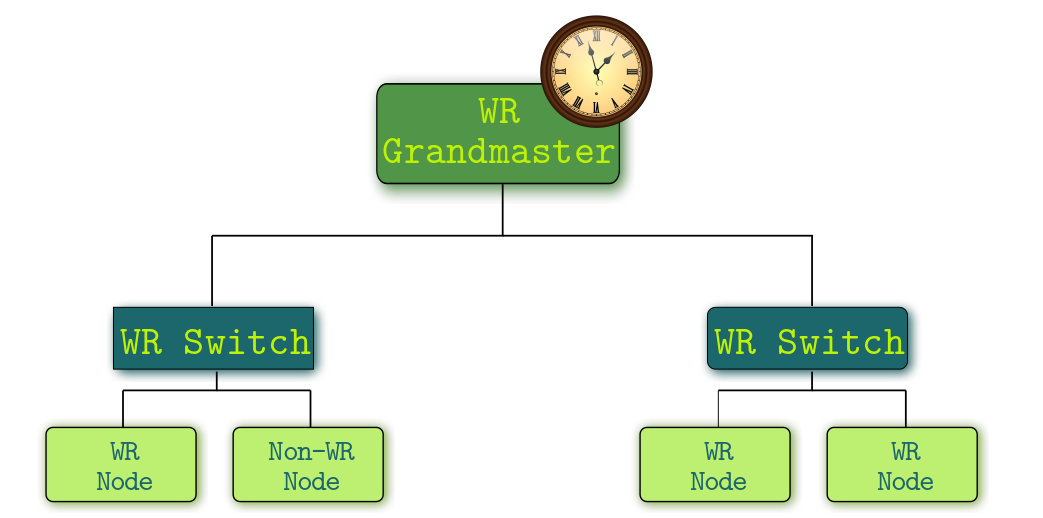
\includegraphics[scale=0.4]{img/wr_hierarchy}
	\caption{The WR network is a tree hierarchy where the root node is the Grand Master that is responsible for distributing the reference time signals. The intermediate elements are WR Switches that acts as Gigabit Ethernet switchers and as Boundary clocks propagating the time signals from the upper layers of the network. Finally, the main purpose of the end-nodes is to provide timing to another specific application.}
	\label{fig:wr_hierarchy}
\end{figure}

\subsection{Selection of WR devices for the SKA telescope} 
\label{subsec:wr-dev}

Regardless of the case of use for the WR technology, it will be needed to 
select a suitable set of WR devices. Most applications distinguish two main 
roles according to a typical WR network: devices which act as BC, and ones 
that act as Ordinary Clocks (OC). Currently, the WRS \cite{ohwr:wrs} is the 
most convenient BC among all the WR devices. 

The WRS has a total of 18 SFP connectors where one could be configured as 
master (downstream) and the rest as slaves (upstream). It is also important to 
remark another I/O ports such as: five coaxial RF connectors and one management 
Ethernet RJ45 connector. Although there are other WR devices that could act as 
BC, the WRS is the most appropriate for a network with a high number of nodes, 
such as is the SKA telescope, because of its high number of SFP slots.

The election of the device acting as OC is not as easy. There are many options 
nowadays, so that, we have analysed three WR devices taking into account the 
specific requirements of the SKA project.

Table \ref{tab:wr_devcomp} contains a comparison between the following three WR 
devices: 
\begin{itemize}
	\item The Simple PCIe FMC carrier (SPEC) \cite{ohwr:spec} is a WR-compliant 
	FMC carrier that supports low pin count (LPC) boards. It includes a 
	Xilinx's Spartan-6 FPGA, an SFP connector and a PCIe interface. It could be 
	used in standalone mode \cite{migueljl-paper-wr-spec}, but due to its 
	limited computational resources, the SPEC is usually used connected to a 
	host PC using the PCIe interface. 
	No coaxial RF connectors are included in the board. This is a major penalty 
	because even for taking the PPS, an external FMC board is needed.
	
	\item The WR Light Embedded Node (LEN) \cite{sevensols:wr_len} is a 
	standalone WR node whose main design principles are: an easiness of use and 
	a good timing performance. It is the first WR node that included the 
	extended version of the WR PTP core (WRPC) architecture, the WR PTP Core 
	Dual Port (WRC2P) \cite{torres2016scalability}. Besides the a second 
	WR-compliant 
	Ethernet interface, the WR-LEN includes three coaxial RF connectors and a 
	Ethernet RJ45 management port. Its design is quite similar to the SPEC 
	board, but with some component upgrades, such as the FPGA (Xilinx's 
	Artix-7).
	
	\item The WR Zynq Embedded Node (ZEN) \cite{sevensols:wr_zen} is another 
	standalone WR node but with many improvements compared to the rest of WR 
	nodes. As in the WR-LEN, the WR implementation corresponds to the WRC2P. 
	That enables a BC configuration as well as OC, or GM configurations. Design 
	is based in a FPGA-SoC from Xilinx (Zynq-7). Thanks to the dual ARM core 
	included on that, the node's design is improved by the use of an Linux-like 
	OS. The board main I/O connectors are: a FMC high pin count (HPC), two 
	SFPs, five coaxial RF and two Ethernet RJ45. The clocking resources include 
	a low-noise oscillator and a flexible PLL schema. That changes are deeply 
	explained in \ref{subsec:hardware}.
\end{itemize}

 \begin{threeparttable}\centering
	\ra{1.1}
	\begin{tabular}{@{} lccc@{}}%\toprule
		& \rotatebox[origin=c]{60}{SPEC} & \rotatebox[origin=c]{60}{WR-LEN}  
		& \rotatebox[origin=c]{60}{WR-ZEN} \\
		\midrule
		\textbf{WR-compliant}\\
		\tab\small{+BC} & \Circle & \CIRCLE & \CIRCLE \\
		\tab\small{+OC} & \CIRCLE & \CIRCLE & \CIRCLE \\
		\tab\small{+GM} & \LEFTcircle & \LEFTcircle & \CIRCLE \\
		\tab\small{+Standalone} & \LEFTcircle & \CIRCLE & \CIRCLE \\
		
		\textbf{RF interfacing}\\
		\tab\small{+PPS output} & \LEFTcircle & \CIRCLE & \CIRCLE \\
		\tab\small{+RF I/O} & \Circle & \CIRCLE & \CIRCLE \\
		\tab\small{+GM input} & \LEFTcircle & \LEFTcircle & \CIRCLE \\
		
		\textbf{Dev. support}\\
		\tab\small{+Monitoring support} & \LEFTcircle & \LEFTcircle & \CIRCLE  
		\\
		\tab\small{+Linux OS} & \Circle & \Circle & \CIRCLE \\
		\tab\small{+Available resources} & \LEFTcircle & \Circle & \CIRCLE \\
		
		\textbf{Extensions}\\
		\tab\small{+FMC connector} & \LEFTcircle & \Circle & \CIRCLE \\ 
		\tab\small{+Redundancy} & \Circle & \LEFTcircle & \LEFTcircle \\
		\bottomrule
	\end{tabular}
	\begin{tablenotes}
		\item \hfill \small{\CIRCLE Fully supported; \LEFTcircle 
		Partially supported; \Circle Not supported}
	\end{tablenotes}
	\caption{Comparison between three WR nodes.}
	\label{tab:wr_devcomp}
\end{threeparttable}

The WR-ZEN is selected among the rest of WR nodes for the SKA telescope. It is 
a standalone node with Linux support that also includes enough I/O ports (RF, 
FMC, etc.) and improved clocking resources looking to fulfil the timing 
requirements of the project.

%WR is designed to be fitted in a Field Programmable Gate Array (FPGA) device 
%due to its flexibility to use in designs in a continuous development state. 
%The 
%source code is mainly written in Hardware Description Languages (HDLs) such as 
%VHDL or Verilog. Moreover, there are several platforms that can implement WR 
%that ensures the vendor-independent feature of WR. The most extended vendor in 
%WR world is Xilinx, some examples of devices using Xilinx's FPGAs are the SPEC 
%board \cite{ohwr:spec} and the WRS \cite{ohwr:wrs}. The other vendor used in 
%WR 
%is Altera. Some examples of boards could be found in \cite{cesar-altera-wr}. 
%The main Intellectual Property (IP) block is the WR PTP core (WRPC) for WR 
%nodes and the Real Time Subsystem (RTS) for WR switches. 

%The utilization of the previous WR-compliant nodes in the SKA system presents 
%an important problem: they are based on PCIe interface cards to be plugged on 
%standard computers, microTCA or VME-64 crates and therefore, a specific 
%computer is necessary to provide the high 
%level software management functionalities. Although most of these cards can be 
%used on stand-alone operation mode, they just use a FPGA device as processing 
%engine and this make very complicated to add new functionalities or standard 
%software tools. The main WR node designs include a soft-microprocessor on the 
%FPGA gateware but it is not 
%enough to fully solve the problem because it requires using complex 
%non-standard firmware programming tools and it normally translates on high 
%time-intensive development effort and makes difficult the upgrade of the 
%system 
%firmware. We have worked with these platform in order to build a sensor 
%network 
%based on the SPEC board allowing the PC-hosted and the standalone modes 
%\cite{migueljl-paper-wr-spec}.

%As a different solution, we present a new platform based on an enhanced 
%technology: The WR Zynq Embedded Node (WR-ZEN) \cite{sevensols:wr_zen}. It is 
%a 
%new generation board that includes a Xilinx Zynq System-on-Chip (SoC) 
%\cite{xilinx:zynq}. The Zynq SoC is composed of a FPGA and a hard ARM dual 
%core 
%microprocessor that can run an application that controls the hardware directly 
%or a standard Operating System such as Linux that can host many different kind 
%of processes at the same time. Moreover, the WR-ZEN allows developing gateware 
%and software on the same chip, tightly integrating performance and flexibility 
%thanks to the use of the co-design strategies. The WR-ZEN offers several 
%advantages over the old WR-compliant nodes (WR-LEN, SPEC or SVEC) such as an 
%enhanced standalone mode with a Linux system that can include high level 
%software capabilities without an external PC and the new clocking circuitry 
%among others. Accordingly, the WR-ZEN has been proposed to be used in the SKA 
%project to implement the PPS distribution system and currently, it is being 
%evaluated as a candidate solution for the SKA PPS distribution system.  

%Next sections will present the proposed system for SKA and the main WR 
%contributions: WR Precision Time Protocol for clock propagation and the 
%generation of PPS signal. 
